%!TEX root = ../bachelor.tex
\chapter{Einleitung}\todo{noch nicht ganz fertig}
Drosophilae melanogaster, im Volksmund auch Fruchtfliege genannt, und ihre Larven sind schon seit Jahrzehnten ein wichtiges Untersuchungsobjekt der Biologie. Sie zeichnen sich aus durch einen schnellen Generationswechsel, eine hohe Nachkommenszahl, eine einfache Chromosomenstruktur und können darüber hinaus leicht gehalten und gezüchtet werden.

%\todo{ghosts lass ich weg, weil ich dafür FTIR erklären müsste}
In den vergangenen Jahren wurden verschiedene Versuchsaufbauten zur Untersuchung des Bewegungsmusters von Drosphilae entwickelt. 
Als problematisch erwies sich, dass das Verhalten der Larven beim Herausnehmen aus ihren Aufzuchtröhrchen, bedingt durch den ausgesetzten Stress, negativ beeinflusst wurde. 
Es wurde daher ein Aufbau entwickelt, in dem die Larven direkt in ihrem Aufzuchtröhrchen beobachtet werden konnten, wie in Abbildung \ref{fig:oldSetup} schematisch dargestellt.
Die Larven befinden sich hierbei in einem Zylinder, der von insgesamt fünf Kameras beobachtet wird, die jeweils an einen Raspberry Pi angeschlossen sind. Die Kameras nehmen nun simultan ein Bild auf, wobei hier eine Synchronisation notwendig ist. Auf Grund der Krümmung des Zylinders, müssen diese nun entsprechend entzerrt werden. Anschließend werden die fünf entzerrten Bilder zu einem Gesamtbild zusammengefügt. 

Um ein besseren Verhältnis zwischen der Anzahl der Kameras und des Aufzuchtgeheges zu erreichen, wäre eine Reduktion der Kameraanzahl wünschenswert. 
Statt eines Zylinders benutzen wir in einem neuen Aufbau einen Kegel, wie in Abbildung \ref{fig:newSetup} zu sehen, und beobachten das Gehege mit einer einzigen Weitwinkelkamera. Eine Synchronisation, sowie ein Zusammenfügen von Einzelbilder, ist hier also nicht mehr notwendig. 
Wie auch bei dem bisherigen Aufbau muss hier jedoch eine Entzerrung durchgeführt werden. Die Larven, die sich am oberen Rand des Kegels befinden scheinen sonst größer, als jene, die sich im unteren Bereich aufhalten. Ein relativer Vergleich der Larven wäre somit nicht möglich. 

In dieser Arbeit werden wir zwei Verfahren zum Entzerren solcher Kegeloberflächen vorstellen, sodass die relative Vergleichbarkeit der Larven gewährleistet ist. 
Dazu werden wir die Kegeloberfläche mit Hilfe einer geeigneten Abbildung auf die Mantelfläche abbilden. 

In Kapitel \ref{ch:theory} dieser Arbeit werden zunächst die notwendigen theoretischen Grundlagen erarbeitet. 
Anschließend stellen wir in Kapitel \ref{ch:method} beide Verfahren zur Entzerrung von Kegeloberflächen vor und erläutern ihre Funktionsweise, woraufhin wir in Kapitel \ref{ch:implementation} auf den implementierten Kalibrierungsassistenten eingehen, der diesen Prozess vereinfachen soll. 
In Kapitel \ref{ch:analysis} stellen wir beide Verfahren gegenüber und untersuchen Einflussfaktoren auf die Präzision und Qualität der Entzerrung. 
Im letzten Kapitel dieser Arbeit ziehen wir ein Fazit und geben einen Ausblick auf mögliche Verbesserungsmaßnahmen für die verwendeten Verfahren.  



\begin{figure}[!htb]
	\centering
	\begin{subfigure}{.5\textwidth}
		\centering
		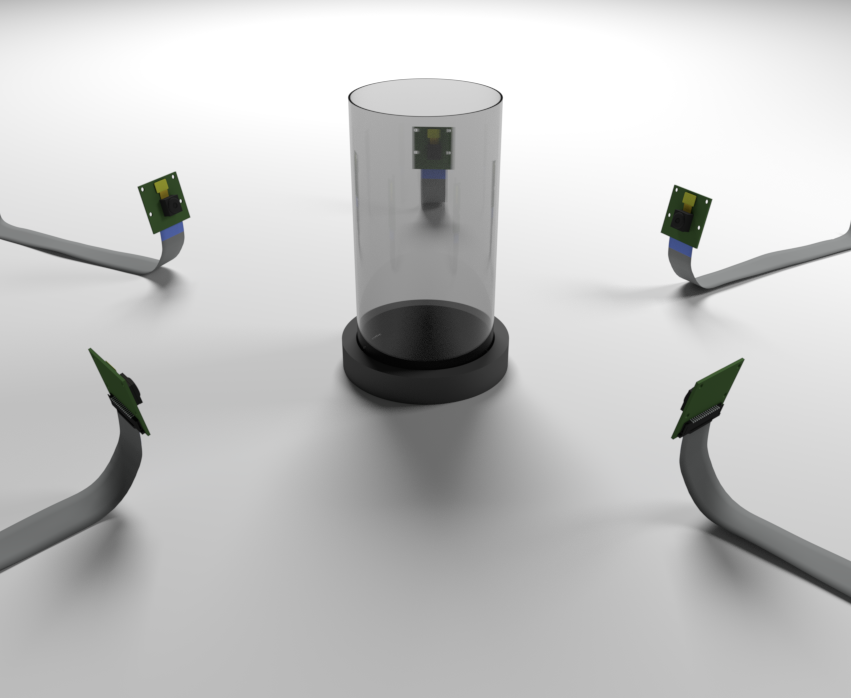
\includegraphics[width=0.95\textwidth]{images/renderCylinder.png}
		\caption{bisheriger Ansatz}
		\label{fig:oldSetup}
	\end{subfigure}%
	\begin{subfigure}{.5\textwidth}
		\centering
		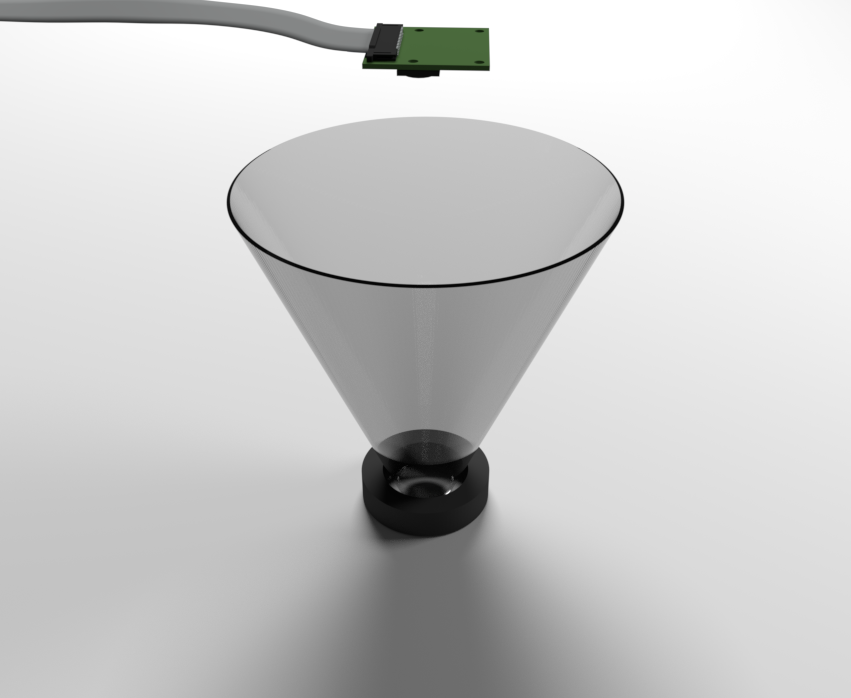
\includegraphics[width=0.95\textwidth]{images/renderCone.png}
		\caption{neuer Ansatz}
		\label{fig:newSetup}
	\end{subfigure}
	\caption{beide Ansätze im Vergleich}
	\label{fig:renderedSetup}
\end{figure}
